\chapter*{Appendix A} 
\label{app:AppendixA}




\chapter*{Appendix B}
\label{app:AppendixB}

In the following we will demonstrate the corrctness of equation \ref{eq:demonstarted}:

\begin{align}
    \varphi_\tau &= 2\pi a \int_{0}^{\infty} \left[ \int_{0}^{\infty} h(t - t') dt' - \int_{0}^{\infty} h(t - \tau - t') dt' \right]^k dt \\
    &= 2\pi a \int_{0}^{\tau} \left[ \int_{0}^{t} h(t - t') dt' \right]^k dt + 2\pi a \int_{\tau}^{\infty} \left[ \int_{0}^{\tau} h(t - t') dt' \right]^k dt,
\end{align}
for different forms of the detuning flux 
\begin{equation}\label{eq:det_flux}
    \Delta f(\Phi) = a\Phi^k
\end{equation}
where $k \in \mathbb{Z}^+$.
From the calculations showed in \ref{eq:phi} we know that the relative phase $\phi_\tau$ for a general form of the detuning flux \ref{eq:det_flux}, with $T_{\text{sep}} = \infty$ is
\begin{equation}\label{eq:phi_here}
    \varphi_{\tau} = 2\pi \int_{0}^{+\infty} a \left[ \left( s(t) - s(t - \tau) \right) \right]^k dt = 2\pi a \int_{0}^{+\infty} \left[ \left( s(t) - s(t - \tau) \right) \right]^k dt
\end{equation}

As hypothesis we know that voltage-to-flux step response of the control line is 
\begin{equation}\label{eq:voltage_to_flux}
    s(t) = \left(1 - e^{-t/\tau} \right) \cdot u(t),
\end{equation} where $u(t)$ is the step function, and that the impulse response is 
\begin{equation}\label{eq:h_def}
    h(t) = \frac{\text{d}s}{\text{d}t}
\end{equation}


If we substitute the expression of $s(t)$ given in \ref{eq:voltage_to_flux} in equation \ref{eq:phi_here} we obtain
\begin{equation}\label{eq:first_step_dem}
    \varphi_{\tau} = 2\pi a \int_{0}^{+\infty} \left[ \int_{0}^{+\infty} h(t - t') dt' - \int_{0}^{+\infty} h(t - \tau - t') dt' \right]^k dt.
\end{equation}

To do we have to show that \begin{enumerate}
    \item \begin{equation}\label{eq:first_dem}
        s(t) = \int_0^{+\infty} h(t-t')dt'
    \end{equation}
    \item \begin{equation}\label{eq:sec_dem}
        s(t-\tau) = \int_{0}^{+\infty} h(t-\tau-t')dt'
    \end{equation}
\end{enumerate}

We start from the demonstration of equation \ref{eq:first_dem}. By definition \ref{eq:h_def} we can write
\begin{equation}\label{eq:first_dem1}
    h(t) = \frac{d}{dt} \left[ \left(1 - e^{-t/\tau} \right) u(t) \right] = \frac{e^{-t/\tau}}{\tau} u(t) + \left(1 - e^{-t/\tau} \right) \delta(t), 
\end{equation}

substituting Eq \ref{eq:first_dem1} in Eq \ref{eq:first_dem} we obtain \begin{equation}
    \int_{0}^{+\infty} h(t - t') dt' = \int_{0}^{+\infty} \frac{e^{-\frac{(t - t')}{\tau}}}{\tau} u(t - t') dt' + \int_{0}^{+\infty} \left(1 - e^{-(t - t')/\tau} \right) \delta(t - t') dt',
\end{equation}
by setting $t'' = t-t'$, $dt''=-dt'$,  we have $t''\rightarrow -\infty$ for $t'\rightarrow +\infty$ and $t''= t$ for $t'= 0$, the integral then becomes
\begin{align}
    \int_{0}^{+\infty} h(t - t') dt' &= \int_{t}^{-\infty} -\frac{e^{-t''/\tau}}{\tau} u(t'') dt'' - \int_{t}^{-\infty} \left(1 - e^{-t''/\tau} \right) \delta(t'') dt'' \\
    &= \int_{-\infty}^{t} \frac{e^{-t''/\tau}}{\tau} u(t'') dt'' + \int_{-\infty}^{t} \left(1 - e^{-t''/\tau} \right) \delta(t'') dt''\\
    &= \int_{0}^{t} \frac{e^{-t''/\tau}}{\tau} u(t'') dt'' + \left(1 - e^{-t''/\tau} \right) \Big|_{t''=0}\\
    &= \left[ -e^{-t''/\tau} u(t'') \right]_{0}^{t} + 0\\
    &= (1 - e^{-t/\tau}) u(t)\\
\end{align}
that concludes the demonstration of Eq \ref{eq:first_dem}.
To demonstrate equation \ref{eq:sec_dem} we starting again by using the definition of $s(t)$ to compute 
\begin{align}
    h(t -t'-\tau) &= \frac{d}{dt} \left[ \left(1 - e^{-(t-t'-\tau)/\tau} \right) u(t-t'-\tau) \right] \\
    &= \frac{e^{-(t-t'-\tau)/\tau}}{\tau} u(t-t'-\tau) + \left(1 - e^{-(t-t'-\tau)/\tau} \right) \delta(t-t'-\tau)\\ \label{eq:sec_dem2}
\end{align}

We can substitute \ref{eq:sec_dem2} in equation \ref{eq:sec_dem} and obtain \begin{equation}
    \int_{0}^{+\infty} h(t - t' - \tau) \, dt' = \int_{0}^{+\infty} \frac{e^{-(t - t' - \tau)/\tau}}{\tau} u(t - t' - \tau) dt' + \int_{0}^{+\infty} \left(1 - e^{-(t - t' - \tau)/\tau} \right) \delta(t - t' - \tau) dt'
\end{equation}
by setting $t'' = t-t'-\tau$, $dt''=-dt'$,  we have $t''\rightarrow -\infty$ for $t'\rightarrow +\infty$ and $t'' = t-\tau$ for $t'= 0$, the integral then becomes
\begin{align}
    \int_{0}^{+\infty} h(t - t'-\tau) dt' &= \int_{-\infty}^{t - \tau} \frac{-e^{-t''/\tau}}{\tau} u(t'') dt'' - \int_{t - \tau}^{\infty} (1 - e^{-t''/\tau}) \delta(t'')\\
    &= \int_{-\infty}^{t - \tau} \frac{e^{-t''/\tau}}{\tau} u(t'') dt'' + \int_{-\infty}^{t - \tau} (1 - e^{-t''/\tau}) \delta(t'')\\
    &= \int_{0}^{t - \tau} \frac{e^{-t''/\tau}}{\tau} u(t'') dt'' + \left(1 - e^{-t''/\tau} \right) \Big|_{t''=0}\\
    &= \left[ - e^{-t''/\tau} u(t'') \right]_{0}^{t - \tau} + 0\\
    &= (1 - e^{-t''/\tau}) u(t'')\\
    &= s(t'') = s(t - t' - \tau)
\end{align}

With this, we demonstrated that 
\begin{equation}
    \varphi_\tau = 2\pi a \int_{0}^{\infty} \left[ \int_{0}^{\infty} h(t - t') \, dt' - \int_{0}^{\infty} h(t - \tau - t') dt' \right]^k dt ,
\end{equation}

We now need to show that 
\begin{align}\label{eq:second_step_dem}
    &2\pi a \int_{0}^{\infty} \left[ \int_{0}^{\infty} h(t - t') dt' - \int_{0}^{\infty} h(t - \tau - t') dt' \right]^k dt\\ 
    &= 2\pi a \int_{0}^{\tau} \left[ \int_{0}^{t} h(t - t') dt' \right]^k dt + 2\pi a \int_{\tau}^{\infty} \left[ \int_{0}^{\tau} h(t - t') \, dt' \right]^k dt.
\end{align}
%
As first step we can try to rewrite the left-hand-side (LHS) in a different way:
\begin{align}
    & 2\pi a \int_{0}^{\infty} \left[ \int_{0}^{\infty} h(t - t') dt' - \int_{0}^{\infty} h(t - \tau - t') dt' \right]^k dt\\ \label{eq:last1}
    &= 2\pi a \int_{0}^{\infty} \left[s(t) -s(t-\tau)\right]^k dt\\ \label{eq:last2}
    &= 2\pi\alpha \int_0^{+\infty} \left[\left(1 - e^{-t/\tau}\right) u(t) - \left(1 - e^{-(t - \tau)/\tau}\right) u(t - \tau)\right]^k dt\\ \label{eq:last3}
    &= 2\pi\alpha \int_0^{\tau} \left[ \left(1 - e^{-t/\tau}\right)u(t)\right]^k dt + 2\pi\alpha \int_{\tau}^{+\infty} \left[ \left(1 - e^{-t/\tau}\right)u(t) - \left(1 - e^{-(t - \tau)/\tau}\right)u(t-\tau) \right]^k dt\\ \label{eq:last4}
    &=  2\pi\alpha \int_0^{\tau} \left[\int_{0}^{\infty} h(t - t') dt' \right]^k dt + 2\pi\alpha \int_{\tau}^{+\infty} \left[ s(t) - s(t-\tau) \right]^k dt\\ \label{eq:last_step}
\end{align}
%
In the first step, to get equation \ref{eq:last2} I simply used the equations \ref{eq:first_dem} and \ref{eq:sec_dem} that were demonstarted before, then by substituting the definition of $s(t)$ we obtain Eq \ref{eq:last3}.
It is possible to separate the integral in equation \ref{eq:last3} by using the definition of $u(t)$ which is null for $t\tau$ and of $u(t-\tau)$ which is null also for $0<t<\tau$, doing this we obtain Eq, \ref{eq:last4}
By substituting back \ref{eq:first_dem} in the first term of equation \ref{eq:last4} we obtain the first term of equation \ref{eq:second_step_dem} which we want to demonstrate, in the second term of the sum instead, we can substitute back the definition of $s(t)$.

At this point we only have to show that for $t>\tau$, which is the interval we are considering in the second term, 
\begin{equation}
    2\pi\alpha \int_{\tau}^{+\infty} \left[ s(t) - s(t-\tau) \right]^k dt = 2\pi a \int_{\tau}^{\infty} \left[ \int_{0}^{\tau} h(t - t') dt' \right]^k dt.
\end{equation}
%
To do this we can first evaluate $s(t)-s(t-\tau)$ in the interval $t>\tau$ so that $u(t)=u(t-\tau)=1$, we have
\begin{equation}\label{eq:final}
    s(t) - s(t-\tau) = 1- e^{-\frac{t}{\tau}} - 1 + e^{-\frac{(t-\tau)}{\tau}} = e^{-\frac{t}{\tau}} \left(e^{\frac{\tau}{\tau}}-1\right) = (e-1)e^{-\frac{t}{\tau}}
\end{equation}
%
If we then compute $\int_{0}^{\tau} h(t - t')dt'$ we obtain
\begin{align}
    \int_{0}^{\tau} h(t-t')dt' &= \int_{0}^{\tau} \left[ \frac{e^{-\frac{(t-t')}{\tau}}}{\tau} u(t-t') - \left(1-e^{-\frac{t-t'}{\tau}}\right)\delta(t-t') \right] dt'\\
    &= \int_{0}^{\tau} \frac{e^{-\frac{(t-t')}{\tau}}}{\tau} u(t-t')dt' \\
    &= \int_{0}^{\tau} \frac{e^{-\frac{(t-t')}{\tau}}}{\tau} dt'\\
    &= \int_{0}^{\tau} \frac{e^{-\frac{t}{\tau}}e^{\frac{t'}{\tau}}}{\tau} = e^{-\frac{t}{\tau}}e^{\frac{t'}{\tau}}\Big|_{0}^{\tau} = e^{\frac{-t}{tau}}(e-1)
\end{align}
which is equal to \ref{eq:final} and then concludes the demonstration.

\chapter{Appendix C}\label{app:AppendixC}

In this appendix are reported the plots of all the Randomized Benchmarking evaluations that have been performed during the optimization using different optimization methods.
\begin{figure}[!h]
    \centering
    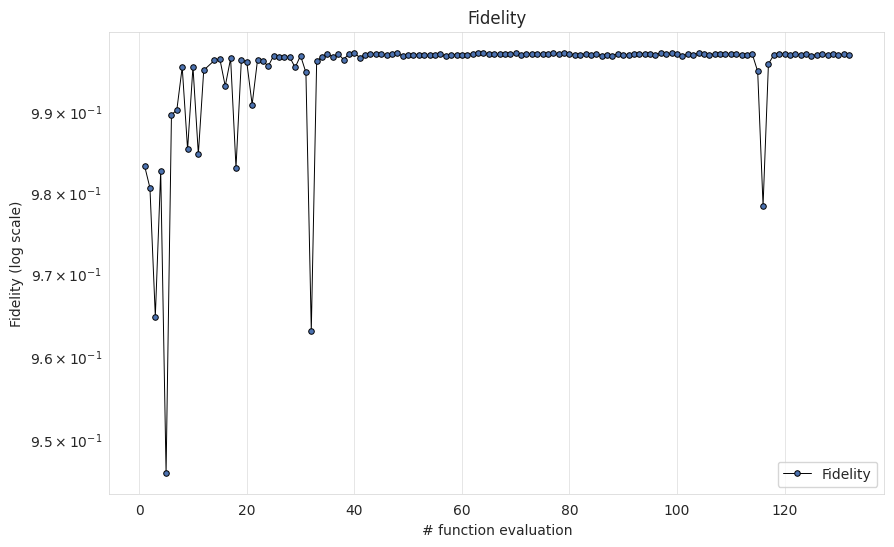
\includegraphics[width=0.75\textwidth]{figures/png/RB_optimization/NM/post_ft_true/NM_complete.png}
    \caption{Plot of the avarge Clifford gate fidielity as a function of the function evauluations.}
    \label{fig:NM}
\end{figure}

\begin{comment}
Possibili esensioni dell'appendice in ordine di priorità:
* resonator spectroscopy s21
* dimostrazione della single gate fidelity dal randomized benchmarking
* spiegare com'è Qibo
* spiegare come ho gestito il passaggio a ruff
\end{comment}